\documentclass[11pt,aspectratio=169]{beamer}
%\documentclass[11pt,aspectratio=169,handout]{beamer}

\usepackage{amsmath}
\usepackage{amsfonts}
\usepackage{amssymb}
\usepackage{graphbox}
\usepackage{sgamevar}
\usepackage{pgfplots}
\usepackage{tikz}
\usepackage{pstricks,pst-node}
\usepackage{bigdelim}
\usepackage{qrcode}
\usepackage[absolute,overlay]{textpos}
\usepackage[ruled,vlined]{algorithm2e}



% alg
\SetKwFor{Repeat}{repeat}{}{}
\SetKwComment{Comment}{$\triangleright$ }{}
\SetCommentSty{textsf}
% pgfplot settings
\usepgfplotslibrary{fillbetween}

% tikz settings
\tikzset{
    invisible/.style={text opacity=1,opacity=0},
    visible on/.style={alt=#1{}{invisible}},
    alt/.code args={<#1>#2#3}{%
      \alt<#1>{\pgfkeysalso{#2}}{\pgfkeysalso{#3}}
    },
  }
\newcommand{\nebox}[2][]{\tikz[baseline=(h.base)]\node[rounded corners,rectangle,draw,line width=0.7pt,text depth=-4.9pt,#1] (h) {#2};}
\usetikzlibrary{arrows}
% Customized colors

\definecolor{ashgrey}{rgb}{0.7, 0.75, 0.71}
\definecolor{lightblue}{RGB}{140, 201, 247}
\definecolor{darkgreen}{RGB}{113, 160, 55}
\definecolor{darkblue}{RGB}{78, 103, 200}
\definecolor{darkpurple}{RGB}{112, 48, 160}

% Hyperlink settings

\hypersetup{colorlinks,urlcolor=darkgreen}

%Beamer settings

\setbeamertemplate{navigation symbols}{} 
\setbeamertemplate{footline}[frame number]
\setbeamertemplate{itemize items}[circle]
\setbeamertemplate{section in toc}[sections numbered]
\setbeamertemplate{subsection in toc}[subsection numbered]

\setbeamercolor{section in toc}{fg=blue}

\AtBeginSection[ ]{
 \begin{frame}{Outline}
  \hypersetup{linkcolor=black}
  \tableofcontents[currentsection]
 \end{frame}
}

% Graphics settings

\graphicspath{{../Figures/}}

% PGFPlot settings

\pgfplotsset{compat = newest}

% Gamesvar settings

\setlength{\arrayrulewidth}{0.91pt}
\renewcommand{\gamestretch}{1.68}
\def\stackedpayoffs#1#2{%
 \begin{array}{c}#1\\[2mm]#2\end{array}
}

% Math

\DeclareMathOperator*{\argmax}{argmax}
\DeclareMathOperator*{\argmin}{argmin}

\newcommand\given[1][]{\:#1\vert\:}
\newtheorem{proposition}{Proposition}

% New environments

\newenvironment{itemizes}[1][1em]{
 \vspace{#1}
 \begin{itemize}
 \setlength{\itemsep}{#1}
}{
 \end{itemize}
}


% Shared title frame

\title{Game-theoretic \\ Foundations of Multi-agent Systems}

\author{Seyed Majid Zahedi}
\titlegraphic{\vspace{-4.2em} 
\includegraphics[height=5.8em]{Logos/logo2}}

\date{} 
\subject{Lecture 1} 
\logo{
\includegraphics[height=5.6em]{Logos/logo1}}
\subtitle{\vspace{2.1em}Lecture 8: Bayesian Games}

\usetikzlibrary{calc}

\begin{document}

 \begin{frame}[plain]
  \titlepage
 \end{frame} 
 
 \section{Introduction and Definitions}
 
  \begin{frame}{Bayesian Games: Games of Incomplete Information}
   \begin{itemizes}[1.2em]
    \item So far, we assumed \alert{all agents know} what game they are playing
    \begin{itemizes}[0.5em]
     \item Number of agents
     \item Actions available to each agent
     \item Utilities associated with each outcome
    \end{itemizes}
    \item In extensive-form games, \alert{taken actions} could be unknown, but \alert{game itself} is
    \item \alert{Bayesian games} allow us to represent uncertainties about game
    \begin{itemizes}[0.5em]
     \item \alert{Commonly known probability distribution} over possible games 
    \end{itemizes}
   \end{itemizes}
  \end{frame}
  
  
  \begin{frame}{Assumptions}
   \begin{itemizes}[1.5em]
    \item All games have \alert{same number of agents} and \alert{same action sets} for each agents
    \item Possible games only differ in agents' utilities for each outcome
    \item Beliefs are \alert{posteriors}, obtained by conditioning common prior on private signals
   \end{itemizes}
  \end{frame}


  \begin{frame}{Bayesian Games: Formal Definition}
   \begin{itemizes}[1.2em]
    \item $N$ is finite set of agents
    \item $A_i$ is set of actions available to agent $i$
    \item $\Theta_i$ is type space of agent $i$
    \item $p: \Theta \mapsto [0, 1]$ is common prior over types
    \item $u_i: A \times \Theta \mapsto \mathbb{R}$ is utility function for agent $i$
   \end{itemizes}
  \end{frame}
  
  
  \begin{frame}{Example I: Bayesian Entry-deterrence Game}
   \begin{itemize}
    \item Firm 1 decides whether to fight, Firm 2 decides whether to enter
    \item Firm 1 knows its cost
    \item Firm 2 is uncertain if 1's cost is 4 w.p. $p$ or 1 w.p. $1-p$
    \item Game takes one of following two forms
    \vspace{1em}
    \begin{center} \scriptsize
     \begin{game}{2}{2}[$\theta_{11}$: High Cost]
      				\> Enter		\>	Stay out	\\
      Build			\> $0, -1$	\>	$2, 0$	\\
      Don't build	\> $2, 1$	\>	$3, 0$
     \end{game}\hspace{2cm}
     \begin{game}{2}{2}[$\theta_{12}$: Low Cost]
      				\> Enter		\>	Stay out	\\
      Build			\> $3, -1$	\>	$5, 0$	\\
      Don't build	\> $2, 1$	\>	$3, 0$
     \end{game}
    \end{center}
    \vspace{1em}
    \item $\Theta_1 = \{\theta_{11}, \theta_{1,2}\}$ and $\Theta_2 = \{\theta_{21}\}$
   \end{itemize}  
  \end{frame}
  
  
  \begin{frame}{Example II}
   \begin{center}
    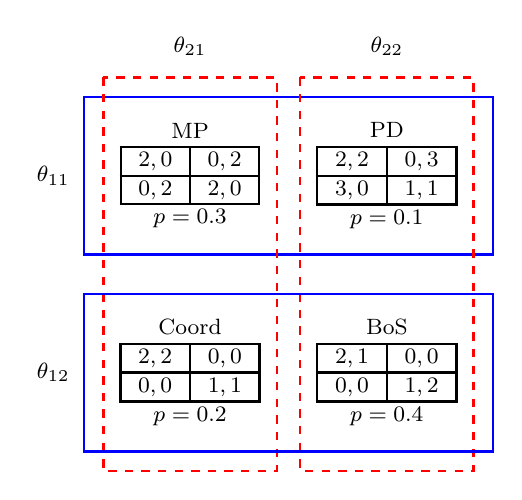
\begin{tikzpicture}[scale=1,font=\footnotesize]
    \tikzstyle{level 1}=[level distance=25mm]
    \tikzstyle{level 2}=[level distance=25mm]
     \node(0){
      \gamemathfalse
      \arrayrulewidth.75pt
      \begin{tabular}[]{|c|c|}
       \multicolumn{2}{c}{MP} \\ \hline
       $2,0$ & $0,2$ \\ \hline
       $0,2$ & $2,0$ \\ \hline
       \multicolumn{2}{c}{$p=0.3$}\\
      \end{tabular}
     }
     child[grow=right]{
      node(1){
       \begin{tabular}[]{|c|c|}
        \multicolumn{2}{c}{PD}\\ \hline
        $2,2$ & $0,3$ \\ \hline
        $3,0$ & $1,1$ \\ \hline
        \multicolumn{2}{c}{$p=0.1$}\\
       \end{tabular}
      }
      child[grow=down]{
       node(2){
        \begin{tabular}[]{|c|c|}
         \multicolumn{2}{c}{BoS}\\ \hline
         $2,1$ & $0,0$ \\ \hline
         $0,0$ & $1,2$ \\ \hline
         \multicolumn{2}{c}{$p=0.4$}\\
        \end{tabular}
       }
       edge from parent[draw=none]
      }
      edge from parent[draw=none]
     }
     child[grow=down]{
      node(3){
       \begin{tabular}[]{|c|c|}
        \multicolumn{2}{c}{Coord}\\ \hline
        $2,2$ & $0,0$ \\ \hline
        $0,0$ & $1,1$ \\ \hline
        \multicolumn{2}{c}{$p=0.2$}\\
       \end{tabular}
      }
      edge from parent[draw=none]
     };
     \node[left,xshift=-40]at(0){$\theta_{11}$};
     \node[left,xshift=-40]at(3){$\theta_{12}$};
     \node[above,yshift=40]at(0){$\theta_{21}$};
     \node[above,yshift=40]at(1){$\theta_{22}$};
     \draw[color=blue,thick]($(0) + (-1.35,1)$) rectangle($(1) +(1.35,-1)$);
     \draw[dashed, color=red,thick] ($(0) + (-1.1,1.25)$)rectangle($(3) +(1.1,-1.25)$);
     \draw[dashed,color=red,thick] ($(1) + (-1.1,1.25)$)rectangle($(2) +(1.1,-1.25)$);
     \draw[color=blue,thick]($(3) + (-1.35,1)$) rectangle($(2) +(1.35,-1)$);
    \end{tikzpicture}
   \end{center}
  \end{frame}
  
  
  \begin{frame}{Types: Discussion}
   \begin{itemizes}
    \item Types encapsulate information possessed by agents that is \alert{not} common knowledge
    \begin{itemize}
     \item E.g., agents' knowledge of their private utility function
    \end{itemize}
    \item Type could also include
    \begin{itemizes}[0.7em]
     \item Agent's beliefs about other agents' utilities
     \item Other agents' beliefs about the agent's own utility
     \item And any other higher-order beliefs
    \end{itemizes}
   \end{itemizes}
  \end{frame}
  
 \section{Strategies and Equilibria}

  \begin{frame}{Strategies}
   \begin{itemizes}[1.2em]
    \item \alert{Before} the game starts, agents only know the common prior
    \item Agent $i$'s strategy is $s_i: \Theta_i \mapsto \Delta(A_i)$ is \alert{contingency plan} for all $\theta_i \in \Theta_i$
    \item $s_i(\theta_i)$ specifies agent $i$'s (mixed) strategy when $i$'s type is $\theta_i$
    \item $s_i(a_i \given \theta_i)$ specifies probability of agent $i$ taking action $s_i$ when $i$'s type is $\theta_i$
    \item Type of agents is \alert{revealed} to them once the game \alert{starts}
    \item Once agents know their type, they follow their strategy for that particular type
   \end{itemizes}
  \end{frame}
  
  
  \begin{frame}{Expected Utilities}
   \begin{itemize}[<+->]
   \setlength{\itemsep}{1.5em}
    \item We can calculate expected utility depending on what agents know
    \item \alert{Ex ante}: Agents only know the common prior on types (before the game starts)
    \item \alert{Interim}: Agents only knows about their own type (after types are reveals)
    \item \alert{Ex post}: Agents know everyone's type (hypothetical -- before they take actions)
   \end{itemize}
  \end{frame}

  \begin{frame}{Expected Utilities (cont.)}
   \begin{itemize}[<+->]
    \item \alert{Ex-post} expected utility (a):
    $$EU_i(s,\theta) = \sum_{a\in A}\left(\prod_{j\in N}s_j(a_j \given \theta_j)\right) u_i(a,\theta)$$
    \item \alert{Interim} expected utility:
    $$EU_i(s,\theta_i) = \sum_{\theta_{-i}\in \Theta_{-i}} p(\theta_{-i} \given \theta_i) EU_i(s, (\theta_i,\theta_{-i}))$$
    \item \alert{Ex-ante} expected utility:
    $$EU_i(s)=\sum_{\theta_i \in \Theta_i} p(\theta_i) EU_i(s,\theta_i) = \sum_{\theta \in \Theta} p(\theta) EU_i(s, \theta)$$
   \end{itemize}
  \end{frame}
  
  
  \begin{frame}{Dominated Strategies}
   \begin{itemizes}[1.5em]
    \item \alert{Ex-ante dominated strategy}: Alternative strategy provides greater ex ante utility regardless of all other agents' strategies
    \item \alert{Interim dominated strategy}: For a given type, alternative strategy provides greater interim utility regardless of all other agents' strategies
   \end{itemizes}
  \end{frame}


  \begin{frame}{Best Response in Bayesian Games}
   \begin{itemize}
   \setlength{\itemsep}{1.2em}
    \item Agent $i$'s \alert{best response} to strategy $s_{-i}$ is
    $$BR_i(s_{-i}) = \; \underset{s_i}{\argmax} \; EU_i(s_i,s_{-i})$$
    \item To play best response, $i$ must know strategy of \alert{all agents} for \alert{each of their types}
    \item Without this information, it is not possible to evaluate $EU_i(s_i, s_{-i})$
   \end{itemize}
  \end{frame}
  
  
  \begin{frame}{Best Response in Bayesian Games (cont.)} \small
   \begin{itemize}[<+->]
    \item Best response is defined based on agent $i$'s \alert{ex ante} expected utility, $EU_i(s_i, s_{-i})$
    \item However, we can rewrite it as
    $$BR_i(s_{-i})= \; \underset{s_i}{\argmax} \; \sum_{\theta_i\in\Theta_i}p(\theta_i)EU_i(s_i,s_{-i},\theta_i)$$
    \item Observe that $EU_i(s_i, s_{-i}, \theta_i)$ \alert{does not depend on} $s_i(\theta_i^\prime)$ for all $\theta_i^\prime \ne \theta_i$
    \item So, maximizing $EU_i(s_i,s_{-i})$ is equal to maximizing $EU_i(s_i,s_{-i},\theta_i)$ for all $\theta_i \in \Theta_i$
    \item Intuitively, if certain action is best after a signal is revealed, it is also the best \alert{conditional plan} devised \alert{ahead of time} for what to do should that signal be received
   \end{itemize}
  \end{frame}
  
  
  \begin{frame}{Bayes-Nash Equilibrium}
    \begin{itemize}
     \item \alert{Bayes-Nash equilibrium (BNE)} is strategy profile $s^*$, such that
     $$s^*_i\in BR_i(s^*_{-i}) ~~\forall i$$
     \item \alert{[Theorem]} Any finite Bayesian game has BNE
    \end{itemize}
  \end{frame}
  
  
  \begin{frame}{Example}
   \begin{center}\scriptsize
    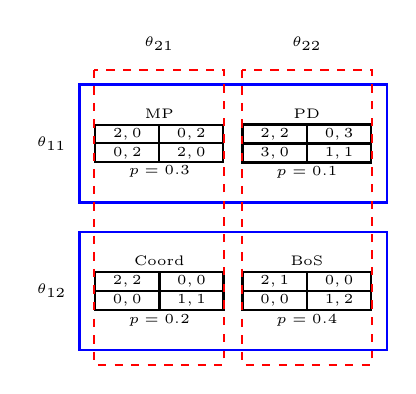
\begin{tikzpicture}[scale=0.75,font=\tiny]
    \tikzstyle{level 1}=[level distance=25mm]
    \tikzstyle{level 2}=[level distance=25mm]
     \node(0){
      \gamemathfalse
      \arrayrulewidth.75pt
      \begin{tabular}[]{|c|c|}
       \multicolumn{2}{c}{MP} \\ \hline
       $2,0$ & $0,2$ \\ \hline
       $0,2$ & $2,0$ \\ \hline
       \multicolumn{2}{c}{$p=0.3$}\\
      \end{tabular}
     }
     child[grow=right]{
      node(1){
       \begin{tabular}[]{|c|c|}
        \multicolumn{2}{c}{PD}\\ \hline
        $2,2$ & $0,3$ \\ \hline
        $3,0$ & $1,1$ \\ \hline
        \multicolumn{2}{c}{$p=0.1$}\\
       \end{tabular}
      }
      child[grow=down]{
       node(2){
        \begin{tabular}[]{|c|c|}
         \multicolumn{2}{c}{BoS}\\ \hline
         $2,1$ & $0,0$ \\ \hline
         $0,0$ & $1,2$ \\ \hline
         \multicolumn{2}{c}{$p=0.4$}\\
        \end{tabular}
       }
       edge from parent[draw=none]
      }
      edge from parent[draw=none]
     }
     child[grow=down]{
      node(3){
       \begin{tabular}[]{|c|c|}
        \multicolumn{2}{c}{Coord}\\ \hline
        $2,2$ & $0,0$ \\ \hline
        $0,0$ & $1,1$ \\ \hline
        \multicolumn{2}{c}{$p=0.2$}\\
       \end{tabular}
      }
      edge from parent[draw=none]
     };
     \node[left,xshift=-30]at(0){$\theta_{11}$};
     \node[left,xshift=-30]at(3){$\theta_{12}$};
     \node[above,yshift=30]at(0){$\theta_{21}$};
     \node[above,yshift=30]at(1){$\theta_{22}$};
     \draw[color=blue,thick]($(0) + (-1.35,1)$) rectangle($(1) +(1.35,-1)$);
     \draw[dashed, color=red,thick] ($(0) + (-1.1,1.25)$)rectangle($(3) +(1.1,-1.25)$);
     \draw[dashed,color=red,thick] ($(1) + (-1.1,1.25)$)rectangle($(2) +(1.1,-1.25)$);
     \draw[color=blue,thick]($(3) + (-1.35,1)$) rectangle($(2) +(1.35,-1)$);
    \end{tikzpicture}
    \vspace{1em}
    \begin{align*}
     EU_2(UD,LR) = \; & \sum_{\theta\in\Theta}p(\theta)EU_2(UD,LR,\theta) \\     
     \visible<2->{= \; & p(\theta_{11},\theta_{2,1})u_2(U,L,\theta_{11},\theta_{2,1}) + p(\theta_{11},\theta_{2,2})u_2(U,R,\theta_{11},\theta_{2,2}) + \\[0.5em]
     & p(\theta_{12},\theta_{2,1})u_2(D,L,\theta_{12},\theta_{2,1}) + p(\theta_{12},\theta_{2,2})u_2(D,R,\theta_{12},\theta_{2,2})\\[0.5em]
     = \; & 0.3 \times 0 + 0.1 \times 3 + 0.2 \times 0 + 0.4 \times 2 = 1.1}
    \end{align*}
   \end{center}
  \end{frame}
  
  
  \begin{frame}{Example (cont.)}
   \begin{itemize}[<+->]
    \item Continuing in this manner, complete payoff matrix can be constructed as
    \vspace{1em}
    \begin{center}
     \hspace{-4.9em}
     \begin{game}{4}{4}
      	\> LL		\> LR		\> RL		\> RR		\\
      UU	\> $2,1$		\> $1,0.7$	\> $1,1.2$	\> $0,0.9$	\\
      UD	\> $0.8,0.2$	\> $1,1.1$ 	\> $0.4,1$	\> $0.6,1.9$	\\
      DU	\> $1.5,1.4$	\> $0.5,1.1$	\> $1.7,0.4$	\> $0.7,0.1$	\\
      DD	\> $0.3,0.6$	\> $0.5,1.5$	\> $1.1,0.2$	\> $1.3,1.1$	\\
     \end{game}
    \end{center}
    \vspace{1em}
    \item Note that row agent's best response to RL is DU
   \end{itemize}
  \end{frame}
  
  
  \begin{frame}{Example (cont.)}
   \begin{itemize}[<+->]
    \item Once row agent receives the signal $\theta_{11}$, we can calculate interim utilities
    \vspace{1em}
    \begin{center}\small
     \hspace{-4.9em}
     \begin{game}{4}{4}
      	\> LL			\> LR		\> RL		\> RR		\\
      UU	\> $2,0.5$		\> $1.5,0.75$	\> $0.5,2$	\> $0,2.25$	\\
      UD	\> $2,0.5$		\> $105,0.75$ 	\> $0.5,2$	\> $0,2.25$	\\
      DU	\> $0.75,1.5$	\> $0.25,1.75$	\> $2.25,0$	\> $1.75,0.25$	\\
      DD	\> $0.75,1.5$	\> $0.25,1.75$	\> $2.25,0$	\> $1.75,0.25$	\\
     \end{game}
    \end{center}
    \vspace{1em}
    \item Row agent's payoffs are now \alert{independent} of action taken upon observing $\theta_{12}$
    \item Note that DU is \alert{still best response} to RL
    \item What has changed is how much better it is compared to other strategies
   \end{itemize}
  \end{frame}


  \begin{frame}{Ex-post Equilibrium}
    \begin{itemize}[<+->]
    \setlength{\itemsep}{1.2em}
     \item Strategy profile $s^*$ is \alert{ex-post equilibrium} if
     $$s^*_i \in \underset{s_i}{\argmax} \; EU_i(s_i,s^*_{-i},\theta) ~~ \forall i, \theta \in \Theta$$
     \item Ex-post equilibrium is similar to \alert{dominant strategy equilibrium}
     \begin{itemizes}[0.7em]
      \item Agents are not assumed to know $\theta$
      \item Even if they knew $\theta$, agents would never want to deviate 
      \item Ex-post equilibrium is \alert{not guaranteed} to exist
     \end{itemizes}
    \end{itemize}
  \end{frame}
  
  
  \begin{frame}{Example: Incomplete Information Cournot}
   \begin{itemizes}[0.7em]
    \item Two firms decide on their production level $q_i \in [0, \infty)$
    \item Price is given by $P(q)$ where $q = q_1 + q_2$
    \item Firm 1 has marginal cost equal to $c$ which is common knowledge
    \item Firm 2's marginal cost is private information
     \begin{itemizes}[0.5em]
      \item $c_L$ with probability $x$ and $c_H$ with probability $(1-x)$, where $c_L < c_H$
     \end{itemizes}
    \item Utility of agents are ($t \in \{L, H\}$ type of firm 2)
     \begin{itemizes}[0.5em]
      \item $u_1((q_1,q_2), t) = q_1 P (q_1, q_2)-c$
      \item $u_2((q_1,q_2), t) = q_2 P (q_1, q_2)-c_t$
     \end{itemizes}
   \end{itemizes}
  \end{frame}
  
  
  \begin{frame}{Example: Incomplete Information Cournot (cont.)}
   \begin{itemizes}
    \item What are firms best responses?
    \begin{align*}
     & B_1(q_L,q_H)=\arg\max_{q\ge 0} \Big(\big(xP(q+q_L)+(1-x)P(q+q_H) - c\big) q\Big) \\
     & B_2^L(q_1)=\arg\max_{q\ge 0} \Big(\big(P(q_1+q) - c_L\big) q\Big) \\
     & B_2^H(q_1)= \arg\max_{q\ge 0} \Big(\big(P(q_1+q) - c_H\big) q\Big)
    \end{align*}
    \item BNE of this game is vector $(q_1^*,q_L^*,q_H^* )$ such that
    \begin{equation*}
     q_1^*\in B_1(q_L^*,q_H^*), q_L^*\in B_2^L(q_1^*), q_H^*\in B_2^H(q_1^*)
    \end{equation*}
   \end{itemizes}
  \end{frame}
  
  \begin{frame}{Example: Incomplete Information Cournot (cont.)}
   \begin{itemize}
    \item For example, if $P(q) = \max(\alpha - q, 0)$, then we have:
    \vspace{1.2em}
    \begin{align*}
     & q_1^*=\frac{1}{3}(\alpha - 2c + x c_L + (1-x) c_H) \\[1.2em]
     & q_L^*=\frac{1}{3}(\alpha - 2c_L + c) - \frac{1}{6}(1 - x)(c_H - c_L) \\[1.2em]
     & q_H^*=\frac{1}{3}(\alpha - 2c_H + c) + \frac{1}{6}x(c_H - c_L)
    \end{align*}
   \end{itemize}
  \end{frame}
  
 \section{Auctions}
 
  \begin{frame}{Multi-agent Resource Allocation}
   \begin{itemize}[<+->]
   \setlength{\itemsep}{0.7em}
    \item Major application of Bayesian games is in \alert{auctions}
    \item Auctions are commonly used to sell (allocate) items to \alert{bidders}
    \item Auctioneers often would like to maximize their \alert{revenue}
    \item Bidders' valuations are usually \alert{unknown} to others and auctioneer
    \item Allocating items to bidders with \alert{highest valuations} is often desirable
    \item Extracting private valuations could be challenging
    \item E.g., giving painting for free to bidder with highest valuation would create incentive for all bidders to overstate their valuations
   \end{itemize}
  \end{frame}


  \begin{frame}{Different Auctions}
   \begin{itemize}[<+->] \small
   \setlength{\itemsep}{1.2em}
    \item \alert{English auction}: bid must be higher than previous one, last bidder wins, pays last bid
    \item \alert{Dutch auction}: price drops until one takes item at that price
    \item \alert{Japanese auction}: price rises, bidders drop out, last bidder wins at price of last dropout
    \item \alert{First-price auction}: bidders bid simultaneously, highest bid wins, winner pays winning bid
    \item \alert{Second-price action}: similar to first price, except that winner pays second highest bid
   \end{itemize}
  \end{frame}

  
  \begin{frame}{Valuations}
   \begin{itemizes}[2em]
    \item \alert{Private valuations}: valuation of each bidder is independent of others' valuations
    \item \alert{Common valuations}: bidders' valuations are correlated to common value
   \end{itemizes}
  \end{frame}


  \begin{frame}{Sealed-bid Auctions (First- and Second-price Auctions)}
   \begin{itemize}[<+->]
   \setlength{\itemsep}{0.5em}
    \item Suppose that there are $N$ bidders and single object for sale
    \item Bidder $i$ has value $v_i$ for the object and bids $b_i$
    \item Utility of bidder $i$ is $v_i - p_i$, where $p_i$ is bidder $i$'s payment
    \item Suppose $v$'s  are drawn \textit{i.i.d.} from $[0,\overline{v}]$ with commonly known CDF $F$
    \item Bidders only know their own realized value (type)
    \item Bidders are risk neutral, maximizing their expected utility
    \item Pure strategy for bidder $i$ is map $b_i:[0,\overline{v} ]\rightarrow \mathbb{R}_+$
   \end{itemize}
  \end{frame}


  \begin{frame}{Second-price Auction}
   \begin{itemize}[<+->]
   \setlength{\itemsep}{1em}
    \item Agent $i$ submit bid $b_i$ simultaneously with other agents
    \item Agent with highest bid wins, and pays second highest bid
    \item Agent $i$'s profit is $v_i - \underset{j\ne i}{\max} \; b_j$ if $i$ wins, and 0 otherwise
    \item \alert{[Proposition]} Truthful bidding (i.e., $b_i = v_i$) is BNE in second price auction
    \item \alert{[Proof]} We need to answer following questions
    \begin{itemizes}[0.7em]
     \item If other bidders bids truthfully, does winner want to change their bid?
     \item If other bidders bids truthfully, does looser want to change their bid?
    \end{itemizes}
   \end{itemize}
  \end{frame}


  \begin{frame}{Truthful Bidding in Second-price Auction}
   \begin{itemizes}
    \item Truthful equilibrium is (weak) \alert{ex-post equilibrium}
    \item I.e., truthful bidding weakly dominates other strategies even if all values are known
    \item \alert{[Proof sketch]} Define maximum bid excluding $i$'s bid as $B_{-i}^* = \underset{j \ne i}{\max} \; b_j$
    \vspace{0.5cm}
    \begin{center}
     \visible<2->{\begin{tikzpicture}[x=0.5cm,y=0.5cm, remember picture, overlay, shift={(-8, -3)}]
      \draw[->,thick] (0,0) -- (3.5,0) node[right] {$B_{-i}^*$};
      \draw[->,thick] (0,0) -- (0,3) node[above] {$u_i(b_i)$};
      \draw[color=red,thick] (0,2) -- (2,0);
      \draw (2,0) node[below, yshift=-2.5] {$v_i$};
     \end{tikzpicture}}
     \hspace{1.5em}
     \visible<3->{\begin{tikzpicture}[x=0.5cm,y=0.5cm, remember picture, overlay, shift={(-2, -3)}]
      \draw[->,thick] (0,0) -- (3.5,0) node[right] {$B_{-i}^*$};
      \draw[->,thick] (0,0) -- (0,3) node[above] {$u_i(b_i)$};
      \draw[color=red,thick] (0,2)  -- (1,1) -- (1,0);
      \draw (1,0) node[below] {$b_i$};
      \draw (2,0) node[below, yshift=-2.5] {$v_i$};
     \end{tikzpicture}}
     \hspace{1.5em}
     \visible<4->{\begin{tikzpicture}[x=0.5cm,y=0.5cm, remember picture, overlay, shift={(4, -3)}]
      \draw[->,thick] (0,0) -- (3.5,0) node[right] {$B_{-i}^*$};
      \draw[->,thick] (0,0) -- (0,3) node[above] {$u_i(b_i)$};
      \draw[color=red,thick] (0,2) -- (2.5,-0.5) -- (2.5,0);
      \draw (2,0) node[below, yshift=-2.5] {$v_i$};
      \draw (2.5,0) node[above] {$b_i$};
     \end{tikzpicture}}
    \end{center}
    \vspace{4em}
    \item<5-> Truthful equilibrium is also the unique BNE
   \end{itemizes}
  \end{frame}


  \begin{frame}{Expected Payment in Second-price Auctions}
   \begin{itemizes}[1em]
    \item Define random variable $y_i = \underset{j \ne i}{\max} \; v_j$
    \begin{itemizes}[0.7em]
     \item CDF of $y_i$ is $G_{y_i}(v) = F(v)^{N-1}$
     \item PDF of $y_i$ is $g_{y_i}(v) = (N-1)f(v)F(v)^{N-2}$
    \end{itemizes}
    \item Expected payment of bidder $i$ with value $v_i$ is given by
    \begin{align*}
     p(v_i) &= P(v_i\text{ wins})\times \mathbb{E}[y_i \given y_i\le v_i]\\[0.7em]
     &= P(y_i\le v_i)\times \mathbb{E}[y_i \given y_i\le v_i]\\[0.7em]
     &= G_{y_i}(v_i)\times G_{y_i}(v_i)^{-1}\int_0^{v_i}yg_{y_i}(y)dy = \; \int_0^{v_i}yg_{y_i}(y)dy
    \end{align*}
   \end{itemizes}
  \end{frame}
  
  
  \begin{frame}{First-price Auctions}
   \begin{itemize}[<+->]
   \setlength{\itemsep}{0.8em}
    \item Utility of agent $i$ is $v_i-b_i$ if $b_i > \underset{j\ne i}{\max} \; b_j$ and zero otherwise
    \item We focus on symmetric (increasing and differentiable) equilibrium strategies $\beta$
    \item Bidder $i$ wins whenever $\underset{j\ne i}{\max} \; \beta(v_j) < b_i$
    \item Since $\beta$ is increasing, we have: $\underset{j\ne i}{\max} \; \beta(v_j) = \beta(\underset{j\ne i}{\max} \; v_j) = \beta (y_i)$
    \item This implies that bidder $i$ wins whenever $y_i < \beta^{-1}(b_i)$
    \item Optimal bid of bidder $i$ is $b_i = \underset{b \ge 0}{\argmax} \; G_{y_i} (\beta^{-1}(b))(v_i - b)$
   \end{itemize}
  \end{frame}


  \begin{frame}{First-price Auctions (cont.)}
   \begin{itemize}
    \item First-order (necessary) \alert{optimality conditions} imply\footnotemark{}:
    $$\frac{g_{y_1}(\beta^{-1}(b_i))}{\beta^\prime(\beta^{-1}(b_i))}(v_i-b_i)-G_{y_i}(\beta^{-1}(b_i))=0$$
    \item In symmetric equilibrium, $b_i = \beta (v_i)$, therefore we have:
     \begin{equation*}
      v_i g_{y_i}(v_i)=\beta^\prime(v_i)G_{y_i}(v_i)+\beta(v_i)g_{y_i}(v_i)=\frac{d}{dv}\big(\beta(v_i)G_{y_i}(v_i)\big)
     \end{equation*}
    \item With \alert{boundary condition} $\beta(0)=0$, we have: 
     \begin{equation*}
      \beta(v_i) = G_{y_i}^{-1}(v_i)\int_0^{v_i}yg_{y_i}(y)dy=\mathbb{E}[y_i \given y_i\le v_i]
     \end{equation*}
   \end{itemize}
   \footnotetext[1]{Derivative of $\beta^{-1}(b)$ is $1/\beta^\prime (\beta^{-1}(b))$.}
  \end{frame}
  
  
  \begin{frame}{Expected Payment in First-price Auctions}
   \begin{itemize}
    \item Expected payment of bidder $i$ with value $v_i$ is:
     \begin{align*}
      p(v_i)&=P(v_i\text{ wins})\times \beta(v_i)\\[0.8em]
      &=P(y_i\le v_i)\times \mathbb{E}[y_i\given y_i\le v_i]\\
      &=G_{y_i}(v_i)\times G_{y_i}(v_i)^{-1}\int_0^{v_i}yg_{y_i}(y)dy =\int_0^{v_i}yg_{y_i}(y)dy
     \end{align*}
    \item This establishes somewhat surprising results that both first and second price auction formats yield \alert{same expected revenue} to auctioneer
   \end{itemize}
  \end{frame}
  
  
  \begin{frame}{Revenue Equivalence}
   \begin{itemize}[<+->]
   \setlength{\itemsep}{1.2em}
    \item In \alert{standard auctions}, item is sold to bidder with highest submitted bid
    \item Suppose that values are \textit{i.i.d} and all bidders are risk neutral
    \item \alert{[Theorem]} Any symmetric and increasing equilibria of any standard auction (such that expected payment of bidder with value zero is zero) yields same expected revenue to auctioneer  
   \end{itemize}
  \end{frame}
  
  
  \begin{frame}{Oil-field Example: Common Values with Correlated Recommendations}
   \begin{itemize}
   \setlength{\itemsep}{0.4em}
    \item Suppose that there are two bidders bidding to lease oil field
    \item Oil field could be worth \$0, \$25M, or \$50M w.p. 0.25, 0.5, and 0.25, respectively
    \item Bidders hire their own consultant to evaluate value of oil field
    \item Bidders get private recommendations, $r_1$ and $r_2$
    \item If field is worth \$0, then $r_1=r_2=L$
    \item If field is worth \$25M, then $r_1=H$, $r_2=L$ or $r_1=L$, $r_2=H$ (both equally likely)
    \item If field is worth \$50M, then $s_1=s_2=H$
    \item Given their private recommendation, how should bidders bid?
   \end{itemize}
  \end{frame}


  \begin{frame}{Oil-field Example: Expected Value}
   \begin{itemize}
    \item What is expected value of oil field if one receives $L$ recommendation?
    \item Given $L$, oil field is worth either \$0 or \$25
    \vspace{1em}
    {\footnotesize
    \begin{align*}
     \visible<2->{&P(\text{\$25M} \given L) = \frac{P(\text{\$25M}) \times P(L \given \text{\$25M})} {P(\text{\$25M}) \times P(L \given \text{\$25M}) + P(\text{\$0}) \times P(L \given \text{\$0})} = \frac{0.5 \times 0.5}{0.5 \times 0.5 + 0.25 \times 1}=0.5\\[1em]}
     \visible<3->{&P(\text{\$0} \given L)=\frac{P(\text{\$0})\times P(L \given \text{\$0})}{P(\text{\$25M})\times P(L \given \text{\$25M})+P(\text{\$0})\times P(L \given \text{\$0})}=\frac{0.25\times 1}{0.5\times 0.5+0.25 \times 1}=0.5\\[1em]}
     \visible<4->{&\mathbb{E}[\text{oil field's value} \given L]=\text{\$25M}\times P(\text{\$25M} \given L)+\text{\$0}\times P(\text{\$0} \given L)=\text{\$12.5M}\\[1em]}
     \visible<5->{&\mathbb{E}[\text{oil field's value} \given H]=\text{\$50M}\times P(\text{\$50M} \given H) + \text{\$25M}\times P(\text{\$25M} \given H)=\text{\$37.5M}}
    \end{align*}}
   \end{itemize}
  \end{frame}
  
  
  \begin{frame}{Oil-field Example: Second-price Auction}
   \begin{itemize}[<+->]
   \setlength{\itemsep}{0.6em}
    \item What is expected utility of bidding \$12.5M upon receiving $L$?
    \begin{itemizes}[0.5em]
     \item With probability 0.5, true value is \$0
     \begin{itemizes}[0.4em]
      \item Other bidder bids \$12.5M
      \item Each bidder wins with probability 0.5 and gets -\$12.5M
     \end{itemizes}
     \item With probability 0.5, true value is \$25M
     \begin{itemizes}[0.4em]
      \item Other bidder bids \$37.7M
      \item Bidder with $L$ loses and gets \$0
     \end{itemizes}
     \item Expected $\text{utility} = 0.5 \times 0.5 \times (-\text{\$12.5M})$
    \end{itemizes}
    \item Bidding \$0 leads to utility \$0 and is \alert{profitable deviation}
    \item \alert{Truthful bidding is not BNE in second-price auction with common values and dependent recommendations}
   \end{itemize}
  \end{frame}
  
  
  \begin{frame}{Winner's Curse}
   \begin{itemizes}
    \item Winning means bidder received highest or \alert{most optimistic} recommendation
    \item Condition on winning, value of item is lower than what recommendation says
    \item Ignoring this leads to paying, on average, \alert{more than} true value of item
    \item To avoid this curse, bidders should assume their recommendation is optimistic
    \item In oil-field example, we can show that the following bidding strategy is BNE
    \begin{itemizes}
     \item Bid 0 upon receiving $L$
     \item Bid \$50M upon receiving $H$  
    \end{itemizes} 
   \end{itemizes}
  \end{frame}
  
  
  \begin{frame}{Oil-field Example II: Common Values and Independent Recommendations}
   \begin{itemizes}[0.6em]
    \item Consider two bidders interested in buying oil field that has part A and B
    \item Each bidder values A and B but is more interested in one of them
    \item Bidders hire their own consultant to evaluate value of their part
    \item Bidder 1 gets private recommendation $r_1$ about value of part A
    \item Bidder 2 gets private recommendation $r_2$ about value of part B 
    \item Suppose that both recommendations are \alert{uniformly distributed} over $[0,1]$
    \item Suppose value of oil field to each bidder is as follows
    \begin{itemizes}[0.4em]
     \item $v_i = a.r_i + b.r_{-i}$ with $a \geq b \geq 0$
     \item Private values are \alert{special case} where $a = 1$ and $b = 0$ 
    \end{itemizes}
   \end{itemizes}
  \end{frame}
  
  
  \begin{frame}{Oil-field Example II: Second-price Auction}
   \begin{itemize}[<+->]
   \setlength{\itemsep}{1.2em}
    \item Similar to previous example, \alert{truthful bidding is not BNE}
    \item Instead, we show that both bidders following $\beta(r_i) = (a + b) r_i$ is BNE
    \item If $-i$ follows this, then probability that $i$ wins by bidding $b_i$ is:
    $$P(\beta(r_{-i}) < b_i) = P((a + b) r_{-i} < b_i) = b_i / (a + b)$$
    \item Bidder $i$'s payment if $i$ wins is $\beta(r_{-i}) = (a + b) r_{-i}$
   \end{itemize}
  \end{frame}
  
  
  \begin{frame}{Oil Field Example II: Second-price Auction (cont.)}
   \begin{itemize}
    \item Expected payment of $i$ condition on $i$ winning is:
    $$\mathbb{E}[(a+b)r_{-i}  \given  r_{-i} < b_i/(a+b)] = b_i/2$$
    \item Expected value of $-i$'s signal condition on $i$ winning is:
    $$\mathbb{E}[r_{-i}  \given  r_{-i} < b_i/(a+b)] = b_i/2(a + b)$$
    \item Expected utility of bidding $b_i$ for recommendation $r_i$ is
    \begin{align*}
     EU(b_i, r_i) & = P(b_i \text{ wins}) \times \left(a.r_i + b.\mathbb{E}[r_{-i}  \given  b_i \text{ wins}] - \mathbb{E}[(a+b)r_{-i}  \given  b_i \text{ wins}]\right) \\
     & = b_i/(a + b) \times (a.r_i + b.b_i/2(a + b) - b_i/2) 
    \end{align*}
    \item Maximizing this with respect to $b_i$ (for given $r_i$) leads to $b_i^* = (a + b) r_i$
   \end{itemize}
  \end{frame}

  \begin{frame}{Oil Field Example II: First-price Auction}
   \begin{itemizes}
    \item Analysis is similar to that of first-price auctions with private values
    \item It can be shown that unique symmetric BNE is for each bidder to bid $\beta(r_i)=(a+b)r_i/2$ 
    \item It can be shown that expected revenue is equal to first price auction
    \item Revenue equivalence principle \alert{continues to hold} for common values  
   \end{itemizes}
  \end{frame}
  
  
 \section{Extensive-form Games of Incomplete-Info}
 
  \begin{frame}{Incomplete Information in Extensive-form Games}
   \begin{itemize}[<+->]
   \setlength{\itemsep}{1.3em}
    \item Incomplete-information games cannot always be represented as \alert{static games}
    \item Extensive-form games can capture explicit order of moves or \alert{dynamic games}
    \item We can use \alert{information sets} to represent what each agent knows
    \item We need to modify BNE to include notion of \alert{perfection} (as in subgame perfection)
   \end{itemize}
  \end{frame}

  \begin{frame}{Equilibrium Concepts}
   \begin{center}
   \renewcommand{\gamestretch}{4}
   \ssualfalse
   \setlength{\fboxrule}{0em}
   \setlength{\fboxsep}{0.5em} 
    \begin{game}{2}{2}[{\Large\rotatebox[origin=c]{90}{Information}}][\Large Timing]
     \> {\footnotesize\fbox{Simultaneous}}	\> {\footnotesize\fbox{Sequential}}	\\
     {\footnotesize\rotatebox[origin=c]{90}{Complete}}	\> Nash	\> SPE \\
     {\footnotesize\rotatebox[origin=c]{90}{Incomplete}} \> Bayesian Nash \> \visible<2->{\alert{Perfect Bayesian}}
    \end{game}
   \end{center}
  \end{frame}
  
  
  \begin{frame}{Extensive-form Games of Incomplete Information: Definition}
   \begin{itemize}
   \setlength{\itemsep}{1.5em}
    \item $N$, $A$, $H$, $Z$, $\alpha$, $\beta$, $\rho$, $u$, and $I$ are the same as extensive-form games
    \item $\Theta_i$ is type space of agent $i$
    \item $p: \Theta \mapsto [0, 1]$ is common prior over types
    \item $u_i: Z \times \Theta \mapsto \mathbb{R}$ is utility function for agent $i$
   \end{itemize}
  \end{frame}
  
 
  \begin{frame}{The ``Nature'' with Chance Moves}
   \begin{itemizes}[1.2em]
    \item To capture common prior, we can add special agent called \alert{Nature}
    \item Nature makes \alert{probabilistic choices}
    \item Nature \alert{does not} have utility function (can be viewed as having constant utility)
    \item Nature has unique strategy of randomizing in \alert{commonly known} way
    \item Agents receive individual signals about Nature's choice
   \end{itemizes}
  \end{frame}
  
  
  \begin{frame}{Example: Kune Poker}
   \begin{center}
    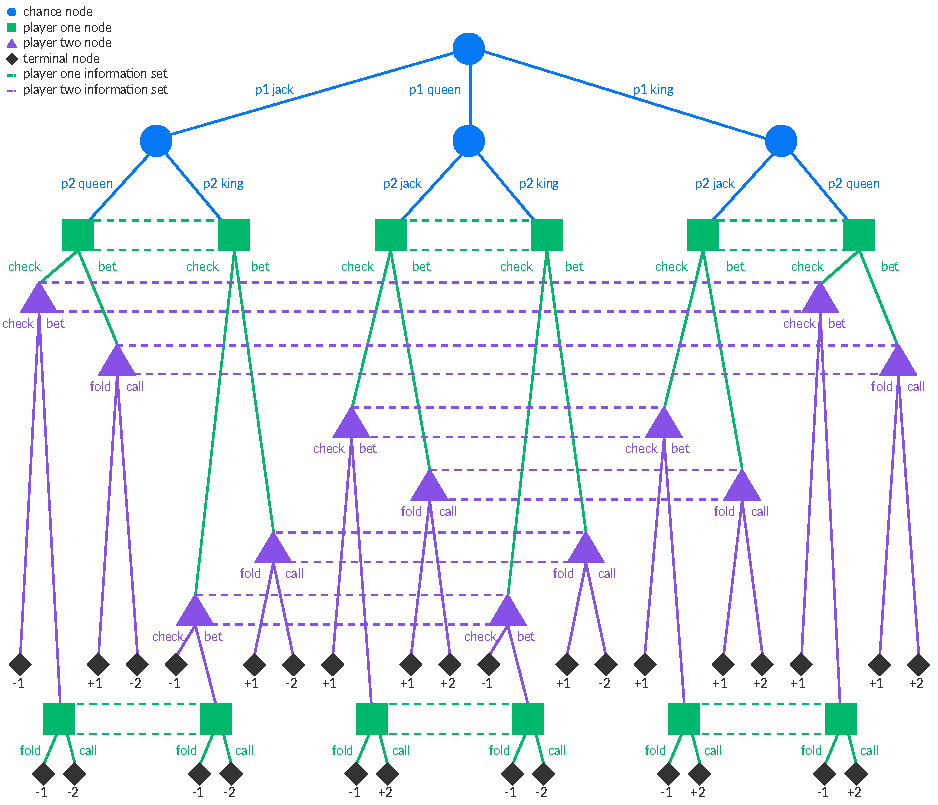
\includegraphics[width=0.6\textwidth]{L8/kuhnPoker}
   \end{center}
  \end{frame}
    
  
  \begin{frame}{Beliefs and Strategies}
   \begin{itemizes}[1.5em]
    \item Agents have \alert{beliefs} about which node they are for each information set (\alert{infoset})
    \item For each infoset, $\mu$ defines \alert{prob. distribution} over all nodes in that infoset
    \item \alert{behavioral strategy}, $s$, maps each infoset prob. distribution over actions
   \end{itemizes}
  \end{frame}
  
  
  \begin{frame}{Requirements for Perfect Bayesian Equilibrium (PBE)}
   \begin{itemize}[<+->]
   \setlength{\itemsep}{1em}
    \item I. Beliefs: In addition to strategy profile $s$, beliefs $\mu$ must be specified
    \item II. \alert{Sequential rationality}: At any infoset, strategy $s$ must be optimal given belief $s$
    \item III. \alert{On-the-path consistency}: For any on-the-equilibrium-path infoset, $\mu$ must be derived from $s$ according to \alert{Bayes' rule}
    \item IV. \alert{Off-the-path consistency}: For any off-the-equilibrium-path infoset, $\mu$ must be derived from $s$ according to Bayes' rule \alert{whenever possible}
   \end{itemize}     
  \end{frame}

  
  \begin{frame}{Weak and Strong PBE}
   \begin{itemize}
   \setlength{\itemsep}{2em}
    \item I-III define \alert{weak PBE}, and I-IV define {strong PBE}
    \item PBE is defined for all extensive-form games with imperfect information
   \end{itemize}
  \end{frame}
  
  
  \begin{frame}{Example I (from Lecture 5)}
   \begin{center}\tiny
    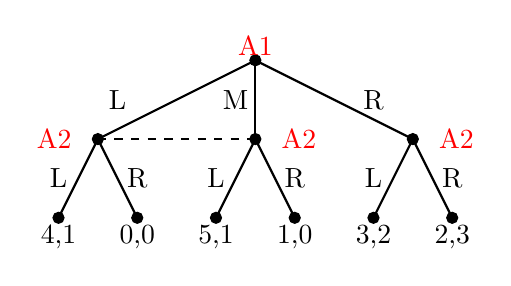
\begin{tikzpicture}[x=0.5cm,y=0.5cm,step=0.5cm]
     \filldraw[black] (5,4) circle (2pt) node[anchor=north, yshift=12pt, color=red]{A1};
     \filldraw[black] (1,2) circle (2pt) node[anchor=east, xshift=-6pt, color=red]{A2};
     \filldraw[black] (5,2) circle (2pt) node[anchor=west, xshift=6pt, color=red]{A2};
     \filldraw[black] (9,2) circle (2pt) node[anchor=west, xshift=6pt, color=red]{A2};
     \filldraw[black] (0,0) circle (2pt) node[] at (0,-0.5) {4,1}; 
     \filldraw[black] (2,0) circle (2pt) node[] at (2,-0.5) {0,0};
     \filldraw[black] (4,0) circle (2pt) node[] at (4,-0.5) {5,1};
     \filldraw[black] (6,0) circle (2pt) node[] at (6,-0.5) {1,0};
     \filldraw[black] (8,0) circle (2pt) node[] at (8,-0.5) {3,2};
     \filldraw[black] (10,0) circle (2pt) node[] at (10,-0.5) {2,3};
     \draw[black, thick] (5,4) -- (1, 2) node[] at (1.5, 3) {L};
     \draw[black, thick] (5,4) -- (5, 2) node[] at (4.5, 3) {M};
     \draw[black, thick] (5,4) -- (9, 2) node[] at (8, 3) {R};
     \draw[black, thick, dashed] (1,2) -- (5, 2); 
     \draw[black, thick] (1,2) -- (0, 0) node[] at (0, 1) {L}; 
     \draw[black, thick] (1,2) -- (2, 0) node[] at (2, 1) {R};
     \draw[black, thick] (5,2) -- (4, 0) node[] at (4, 1) {L};
     \draw[black, thick] (5,2) -- (6, 0) node[] at (6, 1) {R};
     \draw[black, thick] (9,2) -- (8, 0) node[] at (8, 1) {L};
     \draw[black, thick] (9,2) -- (10, 0) node[] at (10, 1) {R};    
    \end{tikzpicture}
   \end{center}
   \begin{itemize}[<+->]\small
   \setlength{\itemsep}{0.5	em}
    \item (R, (R, R)) is NE and SPE, but it is not PBE, why?
    \begin{itemize}
     \item R in A2's left-side infoset is not optimal for any belief of A2
    \end{itemize}
    \item (M, (L, R)) + believing that A2 takes M with probability 1 is weak PBE
    \begin{itemize}
     \item M is best response to (L, R) and (L, R) is best response to M
     \item Off-the-path beliefs are \alert{consistent} with the equilibrium strategy
    \end{itemize}
    \item (M, (L, R)) + believing that A2 takes M with probability 1 is also strong PBE
    \begin{itemize}
     \item Off-the-path beliefs are also consistent (right-side infoset has single node)
    \end{itemize}
   \end{itemize}
  \end{frame}
  
  
  \begin{frame}{Example II: Strong vs. Weak PBE}
   \begin{columns}\footnotesize
    \begin{column}{0.7\textwidth} 
     \begin{itemize}[<+->]
     \setlength{\itemsep}{0.5em}
      \item U is A2's dominant strategy
      \item NE of A2's subgame is (U, R)
      \item (E, U, R) is SPE
      \item (E, U, R) + A3 believing that A2 takes U w.p 1 is PBE (S\&W)
      \item What about (Q, U, L) + A3 believing that A2 takes R w.p. 1?
      \item D is best respond to (U, L) and U is dominant strategy
      \item L is best respond to believing that A2 takes R w.p. 1
      \item So, it is weak PBE, but is it also strong PBE?
      \item No! IV does not hold; A3's belief is \alert{inconsistent} with A2's strategy
     \end{itemize}
    \end{column}
    \begin{column}{0.3\textwidth}
     \begin{center}
      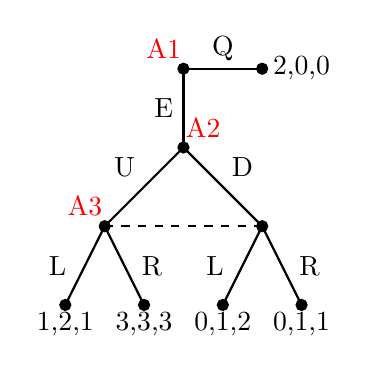
\begin{tikzpicture}[x=0.5cm,y=0.5cm,step=0.5cm]
       \filldraw[black] (3.5, 8) circle (2pt) node[color=red] at (3, 8.5) {A1};
       \filldraw[black] (5.5, 8) circle (2pt) node[] at (6.5, 8) {2,0,0};
       \filldraw[black] (3.5, 6) circle (2pt) node[color=red] at (4, 6.5) {A2}; 
       \filldraw[black] (1.5, 4) circle (2pt) node[color=red] at (1, 4.5) {A3};
       \filldraw[black] (5.5, 4) circle (2pt);
       
       \filldraw[black] (0.5, 2) circle (2pt) node[] at (0.5, 1.5) {1,2,1};
       \filldraw[black] (2.5, 2) circle (2pt) node[] at (2.5, 1.5) {3,3,3};
       \filldraw[black] (4.5, 2) circle (2pt) node[] at (4.5, 1.5) {0,1,2};
       \filldraw[black] (6.5, 2) circle (2pt) node[] at (6.5, 1.5) {0,1,1};
       
       \draw[black, thick] (3.5, 8) -- (5.5,8) node[] at (4.5, 8.5) {Q};
       \draw[black, thick] (3.5, 8) -- (3.5,6) node[] at (3, 7) {E};

       \draw[black, thick] (3.5, 6) -- (1.5,4) node[] at (2, 5.5) {U};
       \draw[black, thick] (3.5, 6) -- (5.5,4) node[] at (5, 5.5) {D};
       
       \draw[black, thick, dashed] (1.5, 4) -- (5.5,4);
       
       \draw[black, thick] (1.5, 4) -- (0.5,2) node[] at (0.3, 3) {L}; 
       \draw[black, thick] (1.5, 4) -- (2.5,2) node[] at (2.7, 3) {R}; 
       \draw[black, thick] (5.5, 4) -- (4.5,2) node[] at (4.3, 3) {L};
       \draw[black, thick] (5.5, 4) -- (6.5,2) node[] at (6.7, 3) {R};
      \end{tikzpicture}
     \end{center}
    \end{column}
   \end{columns}
  \end{frame}
  
  
  \begin{frame}{Example II: Selten's Horse}
   \begin{columns}
    \begin{column}{0.7\textwidth}
     \begin{center}\scriptsize
      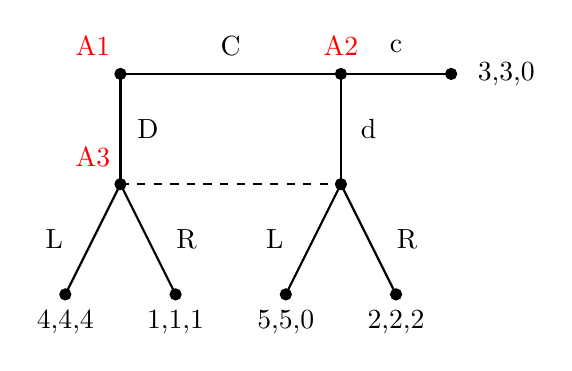
\begin{tikzpicture}[x=0.7cm,y=0.7cm,step=0.7cm]
       \filldraw[black] (1.5, 6) circle (2pt) node[color=red] at (1, 6.5) {A1};
       \filldraw[black] (7.5, 6) circle (2pt) node[] at (8.5, 6) {3,3,0};
       \filldraw[black] (5.5, 6) circle (2pt) node[color=red] at (5.5, 6.5) {A2}; 
       \filldraw[black] (1.5, 4) circle (2pt) node[color=red] at (1, 4.5) {A3};
       \filldraw[black] (5.5, 4) circle (2pt);
       
       \filldraw[black] (0.5, 2) circle (2pt) node[] at (0.5, 1.5) {4,4,4};
       \filldraw[black] (2.5, 2) circle (2pt) node[] at (2.5, 1.5) {1,1,1};
       \filldraw[black] (4.5, 2) circle (2pt) node[] at (4.5, 1.5) {5,5,0};
       \filldraw[black] (6.5, 2) circle (2pt) node[] at (6.5, 1.5) {2,2,2};
       
       \draw[black, thick] (1.5, 6) -- (5.5,6) node[] at (3.5, 6.5) {C};
       \draw[black, thick, dashed] (1.5, 4) -- (5.5,4);
       \draw[black, thick] (1.5, 6) -- (1.5,4) node[] at (2, 5) {D};
       \draw[black, thick] (5.5, 6) -- (5.5,4) node[] at (6, 5) {d};
       \draw[black, thick] (5.5, 6) -- (7.5,6) node[] at (6.5, 6.5) {c};
                     
       \draw[black, thick] (1.5, 4) -- (0.5,2) node[] at (0.3, 3) {L}; 
       \draw[black, thick] (1.5, 4) -- (2.5,2) node[] at (2.7, 3) {R}; 
       \draw[black, thick] (5.5, 4) -- (4.5,2) node[] at (4.3, 3) {L};
       \draw[black, thick] (5.5, 4) -- (6.5,2) node[] at (6.7, 3) {R};
      \end{tikzpicture}
     \end{center}
    \end{column}
    \begin{column}{0.3\textwidth}
     \begin{center}\scriptsize
      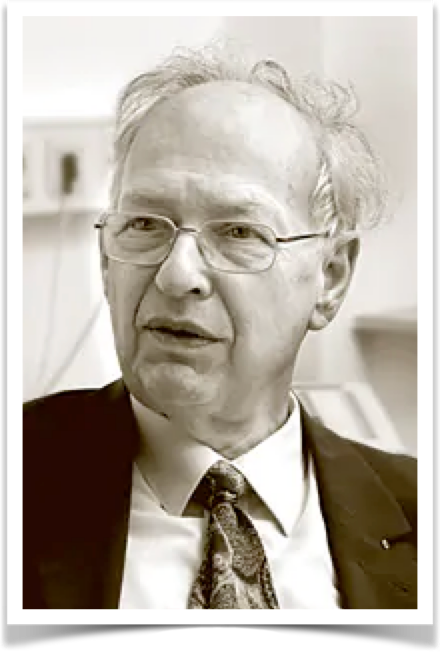
\includegraphics[width=0.6\textwidth]{L8/Selten}\\
      {\scriptsize Reinhard Selten\footnotemark{}\\(1930-2016)}
     \end{center}
    \end{column}
   \end{columns}
   \footnotetext[1]{\tiny Photograph by Stefan Schickler}
  \end{frame}

  
  \begin{frame}{Example II: Selten's Horse (cont.)}
   \begin{center}\scriptsize
    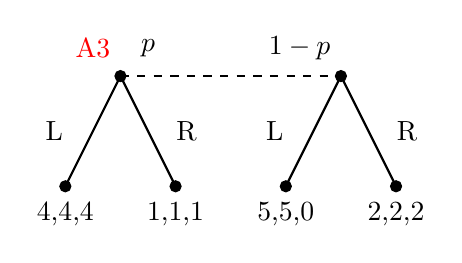
\begin{tikzpicture}[x=0.7cm,y=0.7cm,step=0.7cm]
     \filldraw[black] (1.5, 4) circle (2pt) node[color=red] at (1, 4.5) {A3};
     \filldraw[black] (5.5, 4) circle (2pt);
      
     \filldraw[black] (0.5, 2) circle (2pt) node[] at (0.5, 1.5) {4,4,4};
     \filldraw[black] (2.5, 2) circle (2pt) node[] at (2.5, 1.5) {1,1,1};
     \filldraw[black] (4.5, 2) circle (2pt) node[] at (4.5, 1.5) {5,5,0};
     \filldraw[black] (6.5, 2) circle (2pt) node[] at (6.5, 1.5) {2,2,2};
       
     \draw[black, thick, dashed] (1.5, 4) -- (5.5,4) node[] at (2, 4.5) {$p$} node[] at (4.75, 4.5) {$1-p$};
                     
     \draw[black, thick] (1.5, 4) -- (0.5,2) node[] at (0.3, 3) {L}; 
     \draw[black, thick] (1.5, 4) -- (2.5,2) node[] at (2.7, 3) {R}; 
     \draw[black, thick] (5.5, 4) -- (4.5,2) node[] at (4.3, 3) {L};
     \draw[black, thick] (5.5, 4) -- (6.5,2) node[] at (6.7, 3) {R};
    \end{tikzpicture}
   \end{center}
   \vspace{0.5em}
   \begin{itemize}
    \item A3 believes that left and right nodes are reached w.p. $p$ and $1-p$, respectively
    \item Utility for playing L is $2p$ and $1-p$ for playing R
    \item A3 must play R if $p < 1/3$, R or L if $p = 1/3$, and L if $p > 1/3$
   \end{itemize}
  \end{frame}
  
  
  \begin{frame}{Example II: Selten's Horse (cont.)}
   \begin{center}\scriptsize
    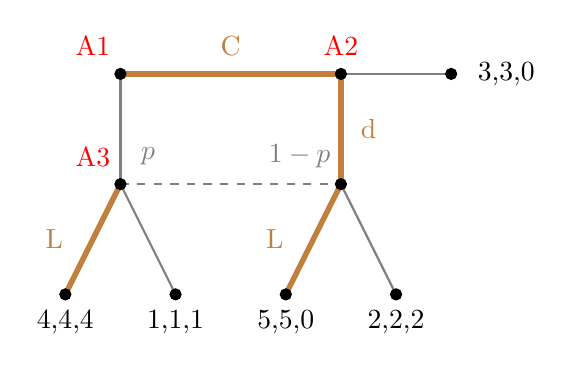
\begin{tikzpicture}[x=0.7cm,y=0.7cm,step=0.7cm]
     \draw[brown, thick, line width=2pt] (1.5, 6) -- (5.5,6) node[] at (3.5, 6.5) {C};
     \draw[gray, thick, dashed] (1.5, 4) -- (5.5,4) node[] at (2, 4.5) {$p$} node[] at (4.75, 4.5) {$1-p$};
     \draw[gray, thick] (1.5, 6) -- (1.5,4);
     \draw[brown, thick, line width=2pt] (5.5, 6) -- (5.5,4) node[] at (6, 5) {d};
     \draw[gray, thick] (5.5, 6) -- (7.5,6);
     
     \draw[brown, thick, line width=2pt] (1.5, 4) -- (0.5,2) node[] at (0.3, 3) {L}; 
     \draw[gray, thick] (1.5, 4) -- (2.5,2); 
     \draw[brown, thick, line width=2pt] (5.5, 4) -- (4.5,2) node[] at (4.3, 3) {L};
     \draw[gray, thick] (5.5, 4) -- (6.5,2);
     
     \filldraw[black] (1.5, 6) circle (2pt) node[color=red] at (1, 6.5) {A1};
     \filldraw[black] (7.5, 6) circle (2pt) node[] at (8.5, 6) {3,3,0};
     \filldraw[black] (5.5, 6) circle (2pt) node[color=red] at (5.5, 6.5) {A2};
     \filldraw[black] (1.5, 4) circle (2pt) node[color=red] at (1, 4.5) {A3};
     \filldraw[black] (5.5, 4) circle (2pt);       
      
     \filldraw[black] (0.5, 2) circle (2pt) node[] at (0.5, 1.5) {4,4,4};
     \filldraw[black] (2.5, 2) circle (2pt) node[] at (2.5, 1.5) {1,1,1};
     \filldraw[black] (4.5, 2) circle (2pt) node[] at (4.5, 1.5) {5,5,0};
     \filldraw[black] (6.5, 2) circle (2pt) node[] at (6.5, 1.5) {2,2,2};
    \end{tikzpicture}
   \end{center}
   \vspace{0.5em}
   \begin{itemize}
    \item Is there any $p$ with which (C, d, L) is weak PBE?
    \item Given (C, d), on-the-path belief for A3 must set $p = 0$
    \item For $p = 0$, A3 must take R, so the answer is \alert{NO}
   \end{itemize}
  \end{frame}
  
  
  \begin{frame}{Example II: Selten's Horse (cont.)}
   \begin{center}\scriptsize
    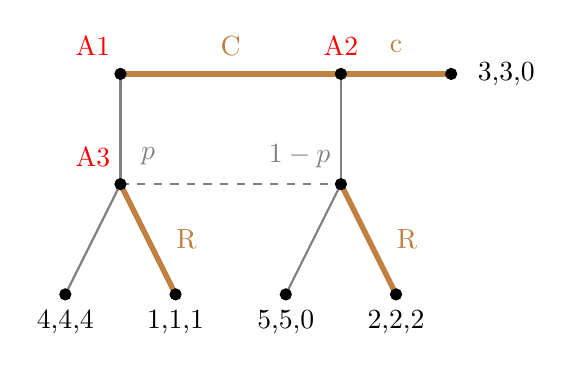
\begin{tikzpicture}[x=0.7cm,y=0.7cm,step=0.7cm]
     \draw[brown, thick, line width=2pt] (1.5, 6) -- (5.5,6) node[] at (3.5, 6.5) {C};
     \draw[gray, thick, dashed] (1.5, 4) -- (5.5,4) node[] at (2, 4.5) {$p$} node[] at (4.75, 4.5) {$1-p$};
     \draw[gray, thick] (1.5, 6) -- (1.5,4);
     \draw[gray, thick] (5.5, 6) -- (5.5,4);
     \draw[brown, thick, line width=2pt] (5.5, 6) -- (7.5,6) node[] at (6.5, 6.5) {c};
     
     \draw[gray, thick] (1.5, 4) -- (0.5,2); 
     \draw[brown, thick, line width=2pt] (1.5, 4) -- (2.5,2) node[] at (2.7, 3) {R}; 
     \draw[gray, thick] (5.5, 4) -- (4.5,2);
     \draw[brown, thick, line width=2pt] (5.5, 4) -- (6.5,2) node[] at (6.7, 3) {R};
     
     \filldraw[black] (1.5, 6) circle (2pt) node[color=red] at (1, 6.5) {A1};
     \filldraw[black] (7.5, 6) circle (2pt) node[] at (8.5, 6) {3,3,0};
     \filldraw[black] (5.5, 6) circle (2pt) node[color=red] at (5.5, 6.5) {A2};
     \filldraw[black] (1.5, 4) circle (2pt) node[color=red] at (1, 4.5) {A3};
     \filldraw[black] (5.5, 4) circle (2pt);       
      
     \filldraw[black] (0.5, 2) circle (2pt) node[] at (0.5, 1.5) {4,4,4};
     \filldraw[black] (2.5, 2) circle (2pt) node[] at (2.5, 1.5) {1,1,1};
     \filldraw[black] (4.5, 2) circle (2pt) node[] at (4.5, 1.5) {5,5,0};
     \filldraw[black] (6.5, 2) circle (2pt) node[] at (6.5, 1.5) {2,2,2};
    \end{tikzpicture}
   \end{center} \small
   \vspace{0.5em}
   \begin{itemize}
    \item Is there any $p$ with which (C, c, R) is weak PBE?
    \item Given (C, c), A3's infoset is off the equilibrium path
    \item \alert{Consistency} does not put any constraint on $p$; \alert{optimality} of R requires $p \le 2/5$
    \item Is (C, c, R) + $p \le 2/5$ strong PBE? Why?
   \end{itemize}
  \end{frame}
  
  
  \begin{frame}{Example III: Signaling Games}
     \begin{itemizes}
      \item \alert{Informed} agent moves first to \alert{signal} some information to uninformed agent
      \item Sending signal is more costly if it conveys false information
      \item E.g., producer provides warranty to signal that its products are unlikely to break
      \item E.g., employees acquire college degree to signal their ability to employers
      \item This is different from sending costless \alert{messages} in \alert{cheap talk} games
      \item Cheap talk is communication between agents that does not directly affect payoffs
      \item E.g., agents message each other on where they want to go in  Battle of the Sexes
     \end{itemizes}
  \end{frame}
  
  
  \begin{frame}{PBE Types in Signaling Games}
   \begin{itemize}[<+->]
   \setlength{\itemsep}{1em}
    \item \alert{Separating}: Informed agent sends distinct signal for each type
    \begin{itemizes}[0.7em]
     \item Signal always reveals sender's type
     \item Receiver's beliefs become deterministic after seeing the signal
    \end{itemizes}
    \item \alert{Pooling}: Informed agent sends the same signal for all types
    \begin{itemizes}[0.7em]
     \item Signal does not give any information to receiver
     \item Receiver's beliefs are not updated after seeing the signal
    \end{itemizes}
    \item \alert{Semi-separating} (a.k.a. partially pooling): Informed agent sends same signal for some types distinct signal for some other types
   \end{itemize}
  \end{frame}
  
  
  \begin{frame}{Simple Poker-like Game: Separating PBE}
   \begin{columns}
    \begin{column}{0.6\textwidth}
     \begin{itemize}[<+->] \scriptsize
     \setlength{\itemsep}{0.7em}
      \item Consider Raising for King and Checking for Jack
      \item What is A2's posterior belief?
      \begin{itemize}\scriptsize
       \item If A1 Raises, then A1 has King w.p. 1
       \item If A1 Checks, then A1 has Jack w.p. 1
      \end{itemize}
      \item What is A2's optimal strategy?
      \begin{itemize}\scriptsize
       \item Fold if A1 Raises, Call if A1 Checks
      \end{itemize}
      \item Given A2's optimal strategy, what is A1's best response?
      \begin{itemize}\scriptsize
       \item Indifferent between Raise and Check if King (1 = 1)
       \item Prefers Raise to Check if Jack (1 $>$ -1)
       \item A1 wants to \alert{deviate} from separating strategy
      \end{itemize}
      \item How about Checking for King and Raising for Jack?
     \end{itemize}
    \end{column}
    \begin{column}{0.4\textwidth}   
     \begin{center}
      \begin{tikzpicture}[x=0.6cm,y=0.6cm,step=0.6cm]
      \tikzstyle{every node}=[font=\tiny]
       \only<1-6>{\draw[black, thick] (0.5, 2) -- (0,0) node[] at (-.25, 1.5) {Call}; 
       \draw[black, thick] (0.5, 2) -- (1,0) node[] at (1.25, 1.5) {Fold};
       \draw[black, thick] (2.5, 2) -- (2,0) node[] at (1.65, 0.5) {Call}; 
       \draw[black, thick] (2.5, 2) -- (3,0) node[] at (3.35, 0.5) {Fold}; 
       \draw[black, thick] (4.5, 2) -- (4,0) node[] at (3.75, 1.5) {Call}; 
       \draw[black, thick] (4.5, 2) -- (5,0) node[] at (5.25, 1.5) {Fold};    
       \draw[black, thick] (6.5, 2) -- (6,0) node[] at (5.65, 0.5) {Call}; 
       \draw[black, thick] (6.5, 2) -- (7,0) node[] at (7.35, 0.5) {Fold};}

       \only<7->{\draw[black, thick] (0.5, 2) -- (0,0) node[] at (-.25, 1.5) {Call}; 
       \draw[brown, thick, line width=2pt] (0.5, 2) -- (1,0) node[] at (1.25, 1.5) {Fold};
       \draw[brown, thick, line width=2pt] (2.5, 2) -- (2,0) node[] at (1.65, 0.5) {Call}; 
       \draw[black, thick] (2.5, 2) -- (3,0) node[] at (3.35, 0.5) {Fold}; 
       \draw[black, thick] (4.5, 2) -- (4,0) node[] at (3.75, 1.5) {Call}; 
       \draw[brown, thick, line width=2pt] (4.5, 2) -- (5,0) node[] at (5.25, 1.5) {Fold};    
       \draw[brown, thick, line width=2pt] (6.5, 2) -- (6,0) node[] at (5.65, 0.5) {Call}; 
       \draw[black, thick] (6.5, 2) -- (7,0) node[] at (7.35, 0.5) {Fold};}

       \filldraw[black] (3.5,6) circle (2pt) node[color=red] at (3.5,7) {Nature};
       \filldraw[black] (1.5,4) circle (2pt) node[color=red] at (1,4.5) {A1};
       \filldraw[black] (5.5,4) circle (2pt) node[color=red] at (6,4.5) {A1};   
       \filldraw[black] (0.5,2) circle (2pt) node[color=red] at (-.5,2) {A2};
       \filldraw[black] (2.5,2) circle (2pt);
       \filldraw[black] (4.5,2) circle (2pt);
       \filldraw[black] (6.5,2) circle (2pt) node[color=red] at (7.5,2) {A2};
       
       \draw[black, thick] (3.5, 6) -- (5.5, 4) node[] at (1, 5.7) {50\% Give I King};
       \draw[black, thick] (3.5, 6) -- (1.5, 4) node[] at (6, 5.7) {50\% Give I Jack};
       \draw[black, thick] (1.5, 4) -- (0.5,2) node[] at (0.3, 3) {Raise}; 
       \draw[black, thick] (1.5, 4) -- (2.5,2) node[] at (2.7, 3) {Check}; 
       \draw[black, thick] (5.5, 4) -- (4.5,2) node[] at (4.3, 3) {Raise};
       \draw[black, thick] (5.5, 4) -- (6.5,2) node[] at (6.7, 3) {Check};       
       \draw[thick, dashed, black] (0.5,2) sin (2.5,2.3);
       \draw[thick, dashed, black] (2.5,2.3) cos (4.5,2);
       \draw[thick, dashed, black] (2.5,2) sin (4.5,2.3);
       \draw[thick, dashed, black] (4.5,2.3) cos (6.5,2);  
        
       \filldraw[black] (0,0) circle (2pt) node[anchor=south, yshift=-20pt]{2};
       \filldraw[black] (1,0) circle (2pt) node[anchor=south, yshift=-20pt]{1};
       \filldraw[black] (2,0) circle (2pt) node[anchor=south, yshift=-20pt]{1};
       \filldraw[black] (3,0) circle (2pt) node[anchor=south, yshift=-20pt]{1};
       \filldraw[black] (4,0) circle (2pt) node[anchor=south, yshift=-20pt]{-2};
       \filldraw[black] (5,0) circle (2pt) node[anchor=south, yshift=-20pt]{1};
       \filldraw[black] (6,0) circle (2pt) node[anchor=south, yshift=-20pt]{-1};
       \filldraw[black] (7,0) circle (2pt) node[anchor=south, yshift=-20pt]{1};
      \end{tikzpicture}
     \end{center}
    \end{column}
   \end{columns}
  \end{frame}
  
  
  \begin{frame}{Simple Poker-like Game: Pooling PBE}
   \begin{columns}
    \begin{column}{0.6\textwidth}
     \begin{itemize}[<+->] \scriptsize
     \setlength{\itemsep}{0.7em}
      \item Consider Raising for both King and Jack
      \item A2's posterior beliefs are the same as prior beliefs
      \begin{itemize}\scriptsize
       \item King w.p. 0.5 and Jack w.p. 0.5
      \end{itemize}
      \item What is A2's optimal strategy on equilibrium path (Raise)?
      \begin{itemize}\scriptsize
       \item Call give 0 (-2 $\times$ 0.5 + 2 $\times$ 0.5), Fold gives -1
       \item A2 prefers Call on the equilibrium path
      \end{itemize}
      \item What is A2's optimal strategy off equilibrium path (Check)?
      \begin{itemize}\scriptsize
       \item Consistency does not put any restriction on beliefs
       \item Consider $p$ for King and $1-p$ for Jack
       \item Call give $-p$ + $1-p$, Fold gives -1 and 
       \item For $p<1$, A2 prefers Call, for $p=1$, A2 is indifferent
      \end{itemize}
     \end{itemize}
    \end{column}
    \begin{column}{0.4\textwidth}   
     \begin{center}
      \begin{tikzpicture}[x=0.6cm,y=0.6cm,step=0.6cm]
      \tikzstyle{every node}=[font=\tiny]
       \only<1-5>{\draw[black, thick] (0.5, 2) -- (0,0) node[] at (-.25, 1.5) {Call}; 
       \draw[black, thick] (0.5, 2) -- (1,0) node[] at (1.25, 1.5) {Fold};
       \draw[black, thick] (2.5, 2) -- (2,0) node[] at (1.65, 0.5) {Call}; 
       \draw[black, thick] (2.5, 2) -- (3,0) node[] at (3.35, 0.5) {Fold}; 
       \draw[black, thick] (4.5, 2) -- (4,0) node[] at (3.75, 1.5) {Call}; 
       \draw[black, thick] (4.5, 2) -- (5,0) node[] at (5.25, 1.5) {Fold};    
       \draw[black, thick] (6.5, 2) -- (6,0) node[] at (5.65, 0.5) {Call}; 
       \draw[black, thick] (6.5, 2) -- (7,0) node[] at (7.35, 0.5) {Fold};}

       \only<6->{\draw[brown, thick, line width=2pt] (0.5, 2) -- (0,0) node[] at (-.25, 1.5) {Call}; 
       \draw[black, thick] (0.5, 2) -- (1,0) node[] at (1.25, 1.5) {Fold};
       \draw[black, thick] (2.5, 2) -- (2,0) node[] at (1.65, 0.5) {Call}; 
       \draw[black, thick] (2.5, 2) -- (3,0) node[] at (3.35, 0.5) {Fold}; 
       \draw[brown, thick, line width=2pt] (4.5, 2) -- (4,0) node[] at (3.75, 1.5) {Call}; 
       \draw[black, thick] (4.5, 2) -- (5,0) node[] at (5.25, 1.5) {Fold};    
       \draw[black, thick] (6.5, 2) -- (6,0) node[] at (5.65, 0.5) {Call}; 
       \draw[black, thick] (6.5, 2) -- (7,0) node[] at (7.35, 0.5) {Fold};}

       \filldraw[black] (3.5,6) circle (2pt) node[color=red] at (3.5,7) {Nature};
       \filldraw[black] (1.5,4) circle (2pt) node[color=red] at (1,4.5) {A1};
       \filldraw[black] (5.5,4) circle (2pt) node[color=red] at (6,4.5) {A1};   
       \filldraw[black] (0.5,2) circle (2pt) node[color=red] at (-.5,2) {A2};
       \filldraw[black] (2.5,2) circle (2pt);
       \filldraw[black] (4.5,2) circle (2pt);
       \filldraw[black] (6.5,2) circle (2pt) node[color=red] at (7.5,2) {A2};
       
       \draw[black, thick] (3.5, 6) -- (5.5, 4) node[] at (1, 5.7) {50\% Give I King};
       \draw[black, thick] (3.5, 6) -- (1.5, 4) node[] at (6, 5.7) {50\% Give I Jack};
       \draw[black, thick] (1.5, 4) -- (0.5,2) node[] at (0.3, 3) {Raise}; 
       \draw[black, thick] (1.5, 4) -- (2.5,2) node[] at (2.7, 3) {Check}; 
       \draw[black, thick] (5.5, 4) -- (4.5,2) node[] at (4.3, 3) {Raise};
       \draw[black, thick] (5.5, 4) -- (6.5,2) node[] at (6.7, 3) {Check};       
       \draw[thick, dashed, black] (0.5,2) sin (2.5,2.3);
       \draw[thick, dashed, black] (2.5,2.3) cos (4.5,2);
       \draw[thick, dashed, black] (2.5,2) sin (4.5,2.3);
       \draw[thick, dashed, black] (4.5,2.3) cos (6.5,2);  
        
       \filldraw[black] (0,0) circle (2pt) node[anchor=south, yshift=-20pt]{2};
       \filldraw[black] (1,0) circle (2pt) node[anchor=south, yshift=-20pt]{1};
       \filldraw[black] (2,0) circle (2pt) node[anchor=south, yshift=-20pt]{1};
       \filldraw[black] (3,0) circle (2pt) node[anchor=south, yshift=-20pt]{1};
       \filldraw[black] (4,0) circle (2pt) node[anchor=south, yshift=-20pt]{-2};
       \filldraw[black] (5,0) circle (2pt) node[anchor=south, yshift=-20pt]{1};
       \filldraw[black] (6,0) circle (2pt) node[anchor=south, yshift=-20pt]{-1};
       \filldraw[black] (7,0) circle (2pt) node[anchor=south, yshift=-20pt]{1};
      \end{tikzpicture}
     \end{center}
    \end{column}
   \end{columns}
  \end{frame}
  
  
  \begin{frame}{Simple Poker-like Game: Pooling PBE (cont.)}
   \begin{columns}
    \begin{column}{0.6\textwidth}
     \begin{itemize}[<+->] \scriptsize
      \item If A2 Calls ($p \le 1)$, what is A1's best response?
      \begin{itemize}\scriptsize
       \item If King, A1 prefers Raise
       \item If Jack, A1 prefers Check
       \item A1 wants to \alert{deviate} from pooling strategy
      \end{itemize}
      \item What if A2 Calls on and Folds off the path (for $p$ = 1)?
      \begin{itemize}\scriptsize
       \item If King, A1 prefers Raise
       \item If Jack, A1 prefers Check
       \item A1 wants to \alert{deviate} from pooling strategy
      \end{itemize}
      \item There is no $p$ for which A1 wants to follow pooling
      \item What about Checking for both King and Jack?
     \end{itemize}
    \end{column}
    \begin{column}{0.4\textwidth}   
     \begin{center}
      \begin{tikzpicture}[x=0.6cm,y=0.6cm,step=0.6cm]
      \tikzstyle{every node}=[font=\tiny]
       \only<1-4>{\draw[brown, thick, line width=2pt] (0.5, 2) -- (0,0) node[] at (-.25, 1.5) {Call}; 
       \draw[black, thick] (0.5, 2) -- (1,0) node[] at (1.25, 1.5) {Fold};
       \draw[brown, thick, line width=2pt] (2.5, 2) -- (2,0) node[] at (1.65, 0.5) {Call}; 
       \draw[black, thick] (2.5, 2) -- (3,0) node[] at (3.35, 0.5) {Fold}; 
       \draw[brown, thick, line width=2pt] (4.5, 2) -- (4,0) node[] at (3.75, 1.5) {Call}; 
       \draw[black, thick] (4.5, 2) -- (5,0) node[] at (5.25, 1.5) {Fold};    
       \draw[brown, thick, line width=2pt] (6.5, 2) -- (6,0) node[] at (5.65, 0.5) {Call}; 
       \draw[black, thick] (6.5, 2) -- (7,0) node[] at (7.35, 0.5) {Fold};}

       \only<5->{\draw[brown, thick, line width=2pt] (0.5, 2) -- (0,0) node[] at (-.25, 1.5) {Call}; 
       \draw[black, thick] (0.5, 2) -- (1,0) node[] at (1.25, 1.5) {Fold};
       \draw[black, thick] (2.5, 2) -- (2,0) node[] at (1.65, 0.5) {Call}; 
       \draw[brown, thick, line width=2pt] (2.5, 2) -- (3,0) node[] at (3.35, 0.5) {Fold}; 
       \draw[brown, thick, line width=2pt] (4.5, 2) -- (4,0) node[] at (3.75, 1.5) {Call}; 
       \draw[black, thick] (4.5, 2) -- (5,0) node[] at (5.25, 1.5) {Fold};    
       \draw[black, thick] (6.5, 2) -- (6,0) node[] at (5.65, 0.5) {Call}; 
       \draw[brown, thick, line width=2pt] (6.5, 2) -- (7,0) node[] at (7.35, 0.5) {Fold};}

       \filldraw[black] (3.5,6) circle (2pt) node[color=red] at (3.5,7) {Nature};
       \filldraw[black] (1.5,4) circle (2pt) node[color=red] at (1,4.5) {A1};
       \filldraw[black] (5.5,4) circle (2pt) node[color=red] at (6,4.5) {A1};   
       \filldraw[black] (0.5,2) circle (2pt) node[color=red] at (-.5,2) {A2};
       \filldraw[black] (2.5,2) circle (2pt);
       \filldraw[black] (4.5,2) circle (2pt);
       \filldraw[black] (6.5,2) circle (2pt) node[color=red] at (7.5,2) {A2};
       
       \draw[black, thick] (3.5, 6) -- (5.5, 4) node[] at (1, 5.7) {50\% Give I King};
       \draw[black, thick] (3.5, 6) -- (1.5, 4) node[] at (6, 5.7) {50\% Give I Jack};
       \draw[black, thick] (1.5, 4) -- (0.5,2) node[] at (0.3, 3) {Raise}; 
       \draw[black, thick] (1.5, 4) -- (2.5,2) node[] at (2.7, 3) {Check}; 
       \draw[black, thick] (5.5, 4) -- (4.5,2) node[] at (4.3, 3) {Raise};
       \draw[black, thick] (5.5, 4) -- (6.5,2) node[] at (6.7, 3) {Check};       
       \draw[thick, dashed, black] (0.5,2) sin (2.5,2.3);
       \draw[thick, dashed, black] (2.5,2.3) cos (4.5,2);
       \draw[thick, dashed, black] (2.5,2) sin (4.5,2.3);
       \draw[thick, dashed, black] (4.5,2.3) cos (6.5,2);  
        
       \filldraw[black] (0,0) circle (2pt) node[anchor=south, yshift=-20pt]{2};
       \filldraw[black] (1,0) circle (2pt) node[anchor=south, yshift=-20pt]{1};
       \filldraw[black] (2,0) circle (2pt) node[anchor=south, yshift=-20pt]{1};
       \filldraw[black] (3,0) circle (2pt) node[anchor=south, yshift=-20pt]{1};
       \filldraw[black] (4,0) circle (2pt) node[anchor=south, yshift=-20pt]{-2};
       \filldraw[black] (5,0) circle (2pt) node[anchor=south, yshift=-20pt]{1};
       \filldraw[black] (6,0) circle (2pt) node[anchor=south, yshift=-20pt]{-1};
       \filldraw[black] (7,0) circle (2pt) node[anchor=south, yshift=-20pt]{1};
      \end{tikzpicture}
     \end{center}
    \end{column}
   \end{columns}
  \end{frame}
  
  
  \begin{frame}{Simple Poker-like Game: Semi-separating PBE}
   \begin{columns}
    \begin{column}{0.6\textwidth}
     \begin{itemize}[<+->] \scriptsize
      \item If King, A1 Raises - If Jack, A1 Raises w.p $x$
      \item What is A2's posterior belief?
      \begin{itemize}\scriptsize
       \item If Check, Jack w.p. 1
       \item If Raise, King w.p. $1/(1+x)$ and Jack w.p. $1/(1+x)$
      \end{itemize}
      \item What is A2's best response if A1 Checks?
      \begin{itemize}\scriptsize
       \item A2 must Call (A2 believes Jack w.p. 1)
      \end{itemize}
      \item A2's strategy should make A1 indifferent if Jack
      \begin{itemize}\scriptsize
       \item Suppose A2 Calls w.p. $y$ if A1 Raises
       \item A1's utility for Raise is $-2y+1-y$
       \item A1's utility for Check is $-1$
       \item $y = 2/3$ makes A1 indifferent
      \end{itemize}
     \end{itemize}
    \end{column}
    \begin{column}{0.4\textwidth}   
     \begin{center}
      \begin{tikzpicture}[x=0.6cm,y=0.6cm,step=0.6cm]
      \tikzstyle{every node}=[font=\tiny]
       \only<1-5>{\draw[black, thick] (0.5, 2) -- (0,0) node[] at (-.25, 1.5) {Call}; 
       \draw[black, thick] (0.5, 2) -- (1,0) node[] at (1.25, 1.5) {Fold};
       \draw[black, thick] (2.5, 2) -- (2,0) node[] at (1.65, 0.5) {Call}; 
       \draw[black, thick] (2.5, 2) -- (3,0) node[] at (3.35, 0.5) {Fold}; 
       \draw[black, thick] (4.5, 2) -- (4,0) node[] at (3.75, 1.5) {Call}; 
       \draw[black, thick] (4.5, 2) -- (5,0) node[] at (5.25, 1.5) {Fold};    
       \draw[black, thick] (6.5, 2) -- (6,0) node[] at (5.65, 0.5) {Call}; 
       \draw[black, thick] (6.5, 2) -- (7,0) node[] at (7.35, 0.5) {Fold};}
       
       \only<6-7>{\draw[black, thick] (0.5, 2) -- (0,0) node[] at (-.25, 1.5) {Call}; 
       \draw[black, thick] (0.5, 2) -- (1,0) node[] at (1.25, 1.5) {Fold};
       \draw[brown, thick, line width=2pt] (2.5, 2) -- (2,0) node[] at (1.65, 0.5) {Call}; 
       \draw[gray, thick] (2.5, 2) -- (3,0); 
       \draw[black, thick] (4.5, 2) -- (4,0) node[] at (3.75, 1.5) {Call}; 
       \draw[black, thick] (4.5, 2) -- (5,0) node[] at (5.25, 1.5) {Fold};    
       \draw[brown, thick, line width=2pt] (6.5, 2) -- (6,0) node[] at (5.65, 0.5) {Call}; 
       \draw[gray, thick] (6.5, 2) -- (7,0);}
       
       \only<8-10>{\draw[black, thick] (0.5, 2) -- (0,0) node[] at (-.25, 1.5) {$y$}; 
       \draw[black, thick] (0.5, 2) -- (1,0) node[] at (1.25, 1.5) {$1-y$};
       \draw[brown, thick, line width=2pt] (2.5, 2) -- (2,0) node[] at (1.65, 0.5) {Call}; 
       \draw[gray, thick] (2.5, 2) -- (3,0); 
       \draw[black, thick] (4.5, 2) -- (4,0) node[] at (3.75, 1.5) {$y$}; 
       \draw[black, thick] (4.5, 2) -- (5,0) node[] at (5.25, 1.5) {$1-y$};    
       \draw[brown, thick, line width=2pt] (6.5, 2) -- (6,0) node[] at (5.65, 0.5) {Call}; 
       \draw[gray, thick] (6.5, 2) -- (7,0);}
       
       \only<11->{\draw[brown, thick, line width=2pt] (0.5, 2) -- (0,0) node[] at (-.25, 1.5) {$\frac{2}{3}$}; 
       \draw[brown, thick, line width=2pt] (0.5, 2) -- (1,0) node[] at (1.25, 1.5) {$\frac{1}{3}$};
       \draw[brown, thick, line width=2pt] (2.5, 2) -- (2,0) node[] at (1.65, 0.5) {Call}; 
       \draw[gray, thick] (2.5, 2) -- (3,0); 
       \draw[brown, thick, line width=2pt] (4.5, 2) -- (4,0) node[] at (3.75, 1.5) {$\frac{2}{3}$}; 
       \draw[brown, thick, line width=2pt] (4.5, 2) -- (5,0) node[] at (5.25, 1.5) {$\frac{1}{3}$};    
       \draw[brown, thick, line width=2pt] (6.5, 2) -- (6,0) node[] at (5.65, 0.5) {Call}; 
       \draw[gray, thick] (6.5, 2) -- (7,0);}

       \draw[black, thick] (3.5, 6) -- (5.5, 4) node[] at (1, 5.7) {50\% Give I King};
       \draw[black, thick] (3.5, 6) -- (1.5, 4) node[] at (6, 5.7) {50\% Give I Jack};
       \draw[brown, thick, line width=2pt] (1.5, 4) -- (0.5,2); 
       \draw[gray, thick] (1.5, 4) -- (2.5,2); 
       \draw[brown, thick, line width=2pt] (5.5, 4) -- (4.5,2) node[black] at (4.3, 3) {$x$};
       \draw[brown, thick, line width=2pt] (5.5, 4) -- (6.5,2) node[black] at (6.7, 3) {$1-x$};

       \filldraw[black] (3.5,6) circle (2pt) node[color=red] at (3.5,7) {Nature};
       \filldraw[black] (1.5,4) circle (2pt) node[color=red] at (1,4.5) {A1};
       \filldraw[black] (5.5,4) circle (2pt) node[color=red] at (6,4.5) {A1};   
       \filldraw[black] (0.5,2) circle (2pt) node[color=red] at (-.5,2) {A2};
       \filldraw[black] (2.5,2) circle (2pt);
       \filldraw[black] (4.5,2) circle (2pt);
       \filldraw[black] (6.5,2) circle (2pt) node[color=red] at (7.5,2) {A2};
              
       \draw[thick, dashed, black] (0.5,2) sin (2.5,2.3);
       \draw[thick, dashed, black] (2.5,2.3) cos (4.5,2);
       \draw[thick, dashed, black] (2.5,2) sin (4.5,2.3);
       \draw[thick, dashed, black] (4.5,2.3) cos (6.5,2);  
        
       \filldraw[black] (0,0) circle (2pt) node[anchor=south, yshift=-20pt]{2};
       \filldraw[black] (1,0) circle (2pt) node[anchor=south, yshift=-20pt]{1};
       \filldraw[black] (2,0) circle (2pt) node[anchor=south, yshift=-20pt]{1};
       \filldraw[black] (3,0) circle (2pt) node[anchor=south, yshift=-20pt]{1};
       \filldraw[black] (4,0) circle (2pt) node[anchor=south, yshift=-20pt]{-2};
       \filldraw[black] (5,0) circle (2pt) node[anchor=south, yshift=-20pt]{1};
       \filldraw[black] (6,0) circle (2pt) node[anchor=south, yshift=-20pt]{-1};
       \filldraw[black] (7,0) circle (2pt) node[anchor=south, yshift=-20pt]{1};
      \end{tikzpicture}
     \end{center}
    \end{column}
   \end{columns}
  \end{frame}
  
  
  \begin{frame}{Simple Poker-like Game: Semi-separating PBE (cont.)}
   \begin{center}
    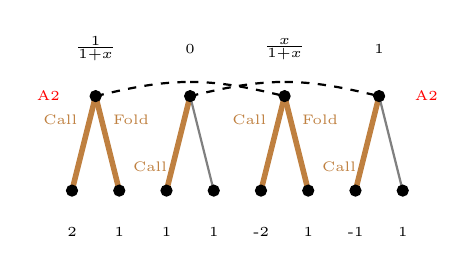
\begin{tikzpicture}[x=0.6cm,y=0.6cm,step=0.6cm]
    \tikzstyle{every node}=[font=\tiny]
     \draw[brown, thick, line width=2pt] (0.5, 2) -- (0,0) node[] at (-.25, 1.5) {Call}; 
     \draw[brown, thick, line width=2pt] (0.5, 2) -- (1,0) node[] at (1.25, 1.5) {Fold};
     \draw[brown, thick, line width=2pt] (2.5, 2) -- (2,0) node[] at (1.65, 0.5) {Call}; 
     \draw[gray, thick] (2.5, 2) -- (3,0); 
     \draw[brown, thick, line width=2pt] (4.5, 2) -- (4,0) node[] at (3.75, 1.5) {Call}; 
     \draw[brown, thick, line width=2pt] (4.5, 2) -- (5,0) node[] at (5.25, 1.5) {Fold};    
     \draw[brown, thick, line width=2pt] (6.5, 2) -- (6,0) node[] at (5.65, 0.5) {Call}; 
     \draw[gray, thick] (6.5, 2) -- (7,0);

     \filldraw[black] (0.5,2) circle (2pt) node[color=red] at (-.5,2) {A2} node[] at (0.5,3) {$\frac{1}{1+x}$};
     \filldraw[black] (2.5,2) circle (2pt) node[] at (2.5,3) {$0$};
     \filldraw[black] (4.5,2) circle (2pt) node[] at (4.5,3) {$\frac{x}{1+x}$};
     \filldraw[black] (6.5,2) circle (2pt) node[color=red] at (7.5,2) {A2} node[] at (6.5,3) {$1$};
       
     \draw[thick, dashed, black] (0.5,2) sin (2.5,2.3);
     \draw[thick, dashed, black] (2.5,2.3) cos (4.5,2);
     \draw[thick, dashed, black] (2.5,2) sin (4.5,2.3);
     \draw[thick, dashed, black] (4.5,2.3) cos (6.5,2);  
        
     \filldraw[black] (0,0) circle (2pt) node[anchor=south, yshift=-20pt]{2};
     \filldraw[black] (1,0) circle (2pt) node[anchor=south, yshift=-20pt]{1};
     \filldraw[black] (2,0) circle (2pt) node[anchor=south, yshift=-20pt]{1};
     \filldraw[black] (3,0) circle (2pt) node[anchor=south, yshift=-20pt]{1};
     \filldraw[black] (4,0) circle (2pt) node[anchor=south, yshift=-20pt]{-2};
     \filldraw[black] (5,0) circle (2pt) node[anchor=south, yshift=-20pt]{1};
     \filldraw[black] (6,0) circle (2pt) node[anchor=south, yshift=-20pt]{-1};
     \filldraw[black] (7,0) circle (2pt) node[anchor=south, yshift=-20pt]{1};
    \end{tikzpicture}
   \end{center}
   \begin{itemize}
    \item $x$ should be set s.t. A2 is indifferent between Call and Fold
    \item If A1 Raises, A2's utility for Call is $(2x-2)/(1+x)$
    \item If A1 Raises, A2's utility for Fold is $-1$
    \item $x = 1/3$ makes A2 indifferent between Call and Fold
   \end{itemize}
  \end{frame}
  
  
  \begin{frame}{Simple Poker-like Game: Final Semi-separating PBE}
   \begin{itemizes}
    \item A1 Raises w.p. 1 if King and w.p. 1/3 if Jack
    \item A1 Checks w.p. 0 if King and w.p. 2/3 if Jack
    \item A2 Calls w.p. 1 if A1 Checks and w.p. 2/3 if A1 Raises
    \item A2 Folds w.p. 0 if A1 Checks and w.p. 1/3 if A1 Raises
    \item If A1 Raises, A2 believes King w.p. 3/4 and Jack w.p. 1/4
    \item If A1 Checks, A2 believes Jack w.p. 1
   \end{itemizes}
  \end{frame}
  

  \begin{frame}{Acknowledgment}
   \begin{itemize}
    \setlength{\itemsep}{1em}
    \item This lecture is a slightly modified version of ones prepared by
    \begin{itemizes}
     \item Asu Ozdaglar \href{https://ocw.mit.edu/courses/electrical-engineering-and-computer-science/6-254-game-theory-with-engineering-applications-spring-2010/index.htm}{[MIT 6.254]}
     \item William Spaniel \href{http://gametheory101.com/courses/game-theory-101/}{Game Theory 101}
    \end{itemizes}
    \item Yiqin Huang helped with importing slides from PowerPoint to \LaTeX
   \end{itemize}
  \end{frame}
  
  
\end{document}
